The data fit at 500 GeV mass point shows relatively high significance and low p-value, which presents a pobability of oberservation.
A signal injection test has been done to check the mass resolution, which constructs a psudo-data containing the MC background and the 500 GeV signal normalised to the fitted signal strength, then a realistic Asimov fit has been done to the pesudo-data at all mass points.

The comparison between the data fit and the pesudo-data fit are shown on the plots below. Figure \ref{fig:injection_1} show the comparisons on the upper limits of the cross section and the observed significance. Figure \ref{fig:injection_2} shows the comparison on the fitted signal sterngth.
The fit results for the 500 GeV mass point are similar, which is expected. However, the expected excess is higher than what are observed in data fit for mass point 400 GeV and 600 GeV. In consequence, the excess at 500 GeV is likely a fluctuation but still has the possibility to be real data.

\begin{figure}

    \begin{center} \setlength{\tabcolsep}{2.5pt}\footnotesize
    \begin{tabular}{cccc}

    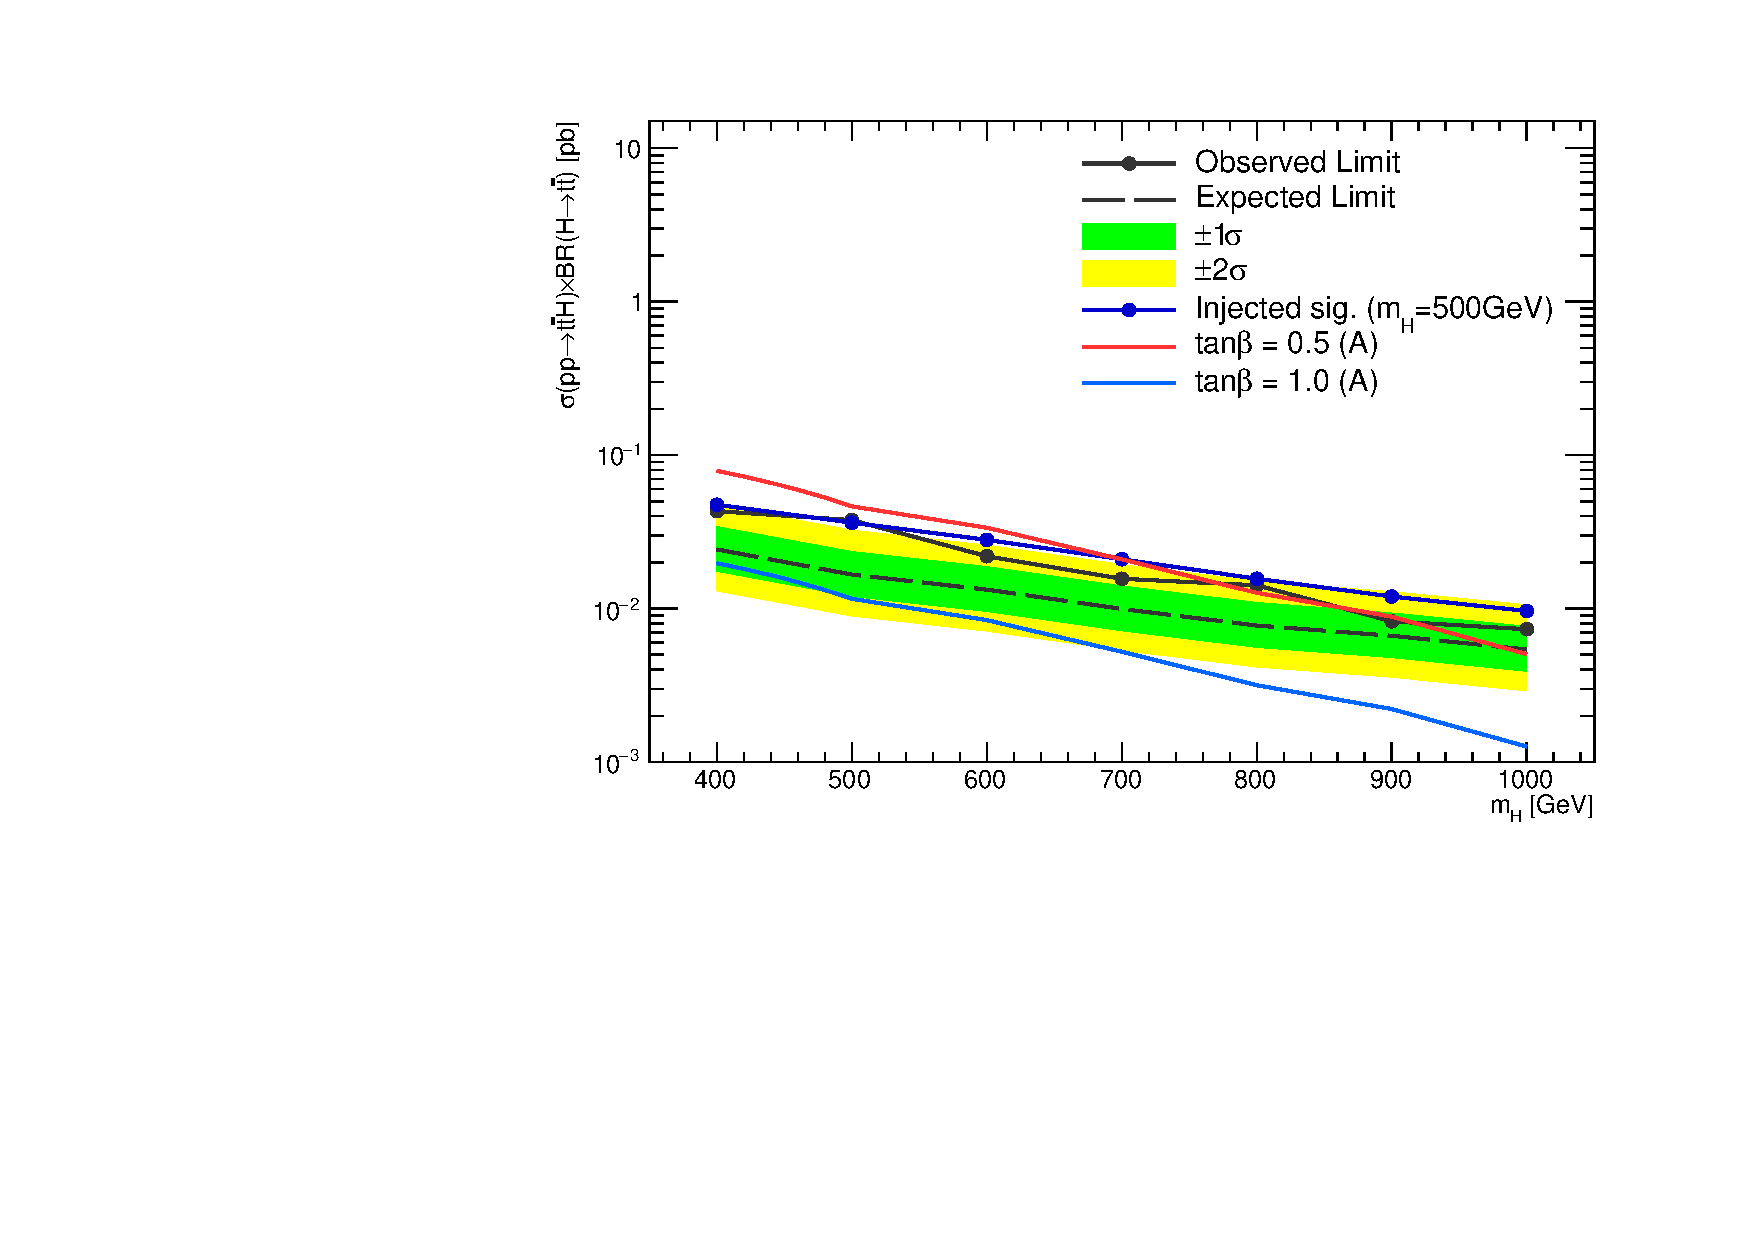
\includegraphics[width=0.45 \textwidth]{figures/injection/lim_injected.pdf} &
    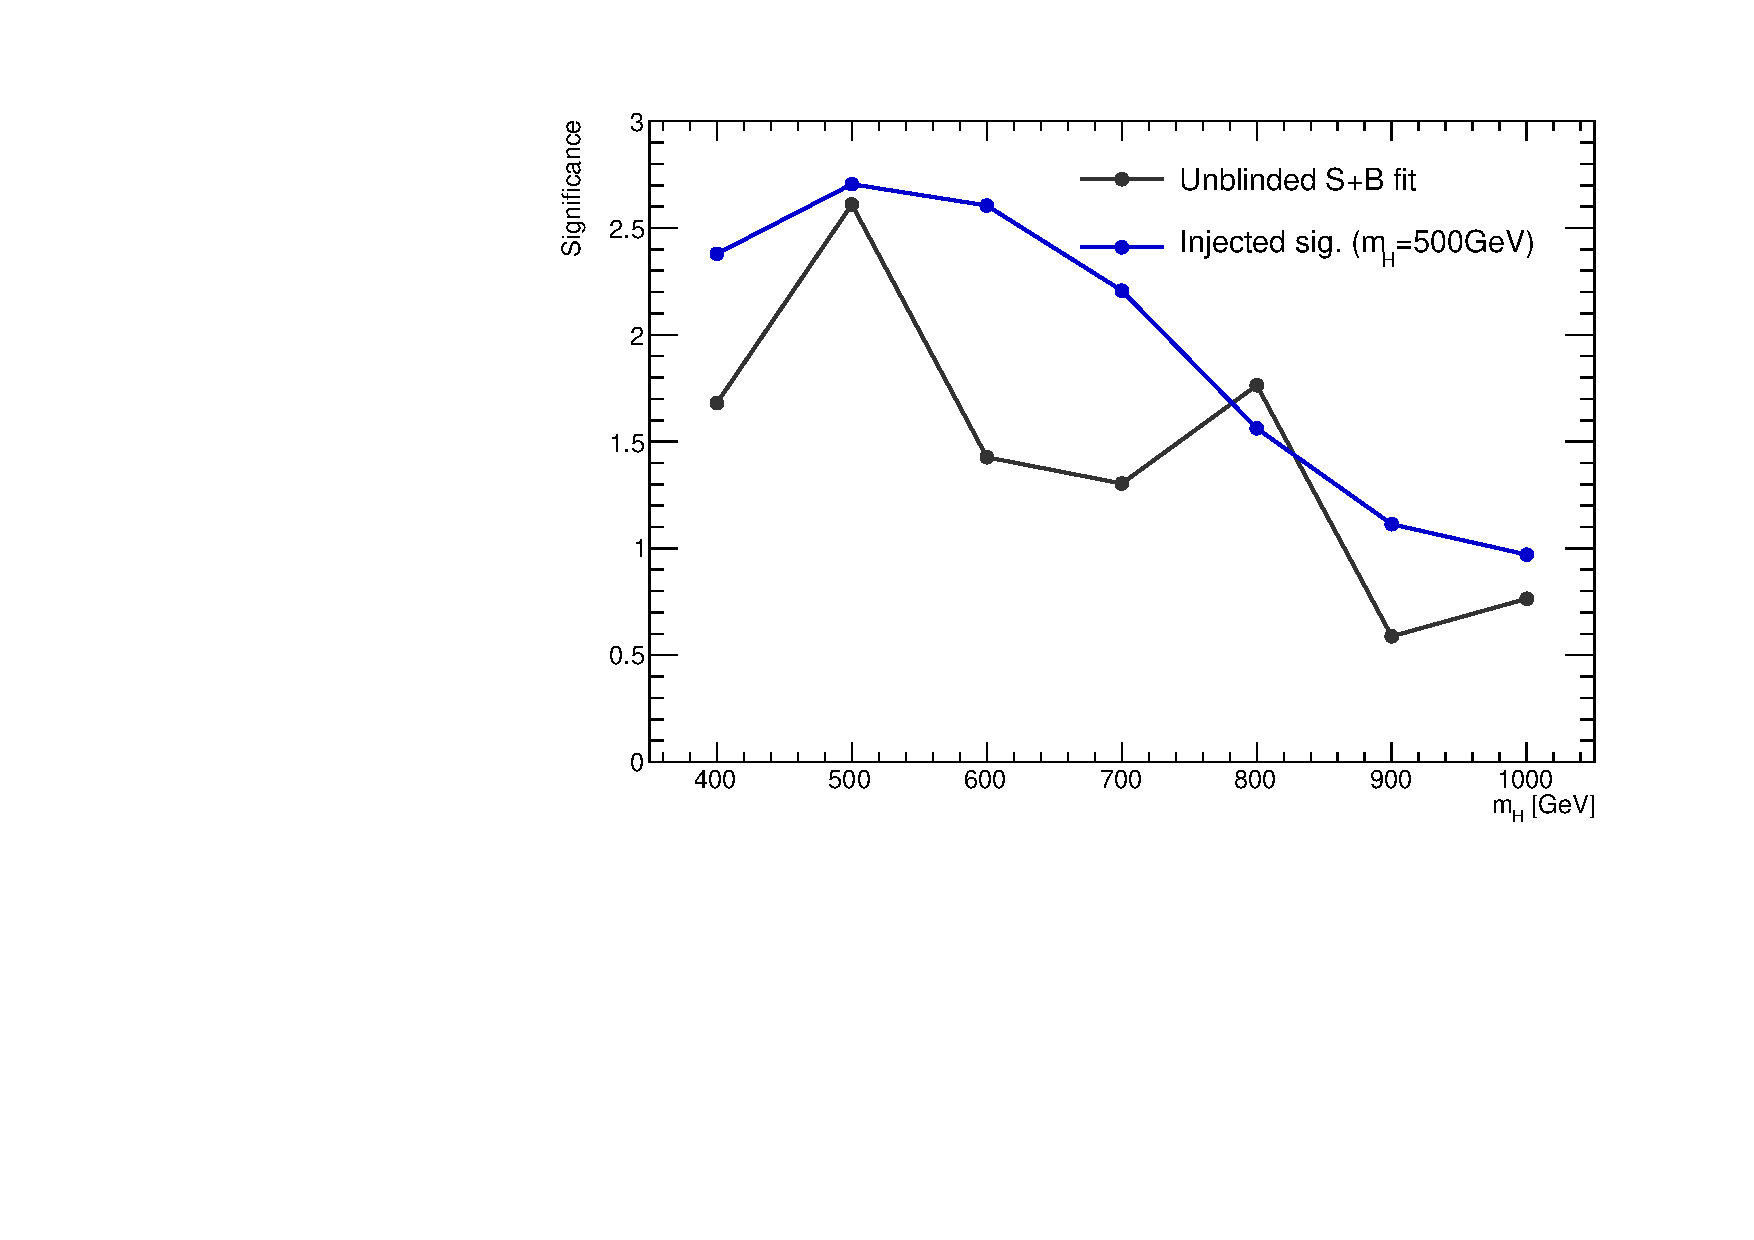
\includegraphics[width=0.45 \textwidth]{figures/injection/sig_comp.pdf}\\

    \end{tabular}
    \end{center}

\caption{\label{fig:injection_1}Comparison of the fit results between data fit and pesudo-data fit. The right plot shows the comparison of the observed upper limit of the cross section, together with the expected upper limt extracted from the data fit. The right plot shows the comparison of the observed significance.}
\end{figure}

\begin{figure}

    \begin{center} \setlength{\tabcolsep}{2.5pt}\footnotesize
    \begin{tabular}{cccc}

    
\includegraphics[width=0.45 \textwidth]{figures/injection/mu_comp.pdf}\\

    \end{tabular}
    \end{center}

\caption{\label{fig:injection_2}Comparison of the fitted signal strength between data fit and pesudo-data fit.}
\end{figure}